\documentclass[twocolumn]{aastex631}

% Packages you've added in

\usepackage{booktabs}
\usepackage{graphicx}


\newcommand{\vdag}{(v)^\dagger}
\newcommand\aastex{AAS\TeX}
\newcommand\latex{La\TeX}
\newcommand{\code}[1]{\texttt{#1}}



\begin{document}

    \title{High Resolution Cross-Correlation Transmission Spectroscopy of KELT-20b}\footnote{Based on data acquired with the Potsdam Echelle Polarimetric and Spectroscopic Instrument (PEPSI) using the Large Binocular Telescope (LBT) in Arizona}

    \author[0009-0001-1459-3738]{Calder Lenhart}
    \affiliation{Department of Astronomy, The Ohio State University \\ 4055 McPherson Laboratory, 140 West 18th Avenue \\ Columbus, OH 43210}

    \author[0000-0002-5099-8185]{Marshall C. Johnson}
    \affiliation{Department of Astronomy, The Ohio State University \\ 4055 McPherson Laboratory, 140 West 18th Avenue \\ Columbus, OH 43210}

    \author{Ji Wang}
    \affiliation{Department of Astronomy, The Ohio State University \\ 4055 McPherson Laboratory, 140 West 18th Avenue \\ Columbus, OH 43210}

    \author[0000-0002-8823-8237]{Anusha Pai Asnodkar}
    \affiliation{Department of Astronomy, The Ohio State University \\ 4055 McPherson Laboratory, 140 West 18th Avenue \\ Columbus, OH 43210}

    \author{Sydney Petz}
    \affiliation{Department of Astronomy, The Ohio State University \\ 4055 McPherson Laboratory, 140 West 18th Avenue \\ Columbus, OH 43210}

    \author[0000-0002-6192-6494]{Klaus Stassmeier}
    \affiliation{Leibniz-Institut für Astrophysik Potsdam, An der Sternwarte 16 D-14482 Potsdam, Germany}

    \author[0000-0002-0551-046X]{Ilya Ilyin}
    \affiliation{Leibniz-Institut für Astrophysik Potsdam, An der Sternwarte 16 D-14482 Potsdam, Germany}


    \begin{abstract}
        Ultra hot Jupiters (UHJs) are prime observational candidates owing to their proximity to their host stars. They have large radii with inflated envelopes, high temperatures, and short orbital periods --- allowing for frequent observations with strong signal clarity. Using the PEPSI high resolution spectrograph on the LBT, we present a complete inventory of detections, line velocities, and phase-resolved dynamics for atomic and molecular species in KELT-20b's atmosphere. We do not detect any molecular species, and we confirm previous atomic detections of Mg I, Fe I, Fe II, Na I, Cr II, and C II. We present a novel detection of Cu I and novel tentative detections of Cr I, Co I, Zn I, Ca I, and Ti II.
    \end{abstract}

    \keywords{}


    \section{Introduction}\label{sec:intro}



    \section{Observations}\label{sec:Observations}
        We obtained our data with the Potsdam Echelle Polarimetric and Spectroscopic Instrument (PEPSI)\citep{Strassmeier2015} on the Large Binocular Telescope (LBT). We utilized the PEPSI 5 III+V bandpass, with wavelength coverage of 4800--5441\AA\ and 6278--7419\AA\, henceforth referred to the blue arm and arm respectively, with resolution ${\mathcal{R} = 130000}$. We list the key observation parameters in Table~\ref{tab:observation_details}.  %perhaps inlcude note about how many of the 23 spectra were in-transit vs out of transit
        We reduced this observation using the Spectroscopic Data Systems (SDS) Pipeline.

        \begin{deluxetable}{lc}
            \tablecaption{Observation details for 2019 May 4 transit.\label{tab:observation_details}}
            \tablehead{
                \colhead{\textbf{Parameter}} & \colhead{\textbf{Value}}
            }
            \startdata
            $N_{\text{spec}}$ & 23 \\
            Exp. Time (s) & 600 \\
            Airmass Range & 1.00--2.01 \\
            Phases Covered & $-0.023$--0.034 \\
            $S/N_{\text{blue}}$ & 288 \\
            $S/N_{\text{red}}$ & 308 \\
            \enddata
        \end{deluxetable}
        

        
    \section{Methodology}\label{sec:Methodology}

        \subsection{Model Spectra}\label{subsec:Model Spectra}
            We generate model transmission spectra, ranging from 3850--7500\AA\ with 0.01\AA\ spacing, with the \code{petitRADTRANS} package~\citep{petitRADTRANS}, as shown in Figure~\ref{fig:main-spectra}. These spectra encompass the PEPSI CD III+V bandpass. We assume stellar and planetary parameters from~\citet{Lund2017}, listed in Table~\ref{tab:parameters_summary}. We select a P-T profile given by Equation (29) of~\citet{Guillot2010} with best-fit parameters $\gamma = 30$ and $K_{IR} = 0.04$ as obtained in a grid search in~\citet{Johnson2023}. While these parameters were derived using emission spectra, transmission spectra are less sensitive to detailed vertical temperature structures~\citep{Kesseli2020}. Since our analysis concerns the atmosphere's kinematics as opposed to chemistry, we deem the same profile sufficient for this analysis. 
            We calculate volume mixing ratios (VMRs) for each species using the \code{PyFastChem} equilibrium chemistry model~\citep{Stock2018, Stock2022, Kitzmann2023}, assuming solar abundances~\citep{Asplund2021} and the aforementioned P-T profile. We assume that quenching, the mechanism by which atmospheric abundances diverge from those predicted by chemical equilibrium at a certain pressure, occurs at 1 bar. Thus, we approximate each species' VMR as equal to its maximum VMR at 1 bar, calculated by \code{PyFastChem}~\citep{Johnson2023,Petz2023}. We also set the VMRs of ionized species equal to those of their neutral counterparts to simplify our analysis. Opacities were sourced from the~\code{petitRADTRANS} database, with missing entries supplemented from the DACE Opacity Database\footnote{\url{https://dace.unige.ch/opacityDatabase/}}, converted to \code{petitRADTRANS}-compatible format (P. Mollière, private communication).~\code{peitRADTRANS} sources its atomic opacities from the Kurucz line list, and we ensured the DACE opacities---Na I and Co I---came from the same line list.~\footnote{\url{http://kurucz.harvard.edu/}}
        
            \begin{deluxetable*}{l l c c}\label{tab:parameters_summary}
                \tablecaption{This table summarizes the planetary and stellar parameters relevant to our analysis. Sources: a:~\citet{Lund2017}; b:~\citet{Johnson2023}.}
                \tablehead{
                    \colhead{\textbf{Description}} & \colhead{\textbf{Parameter}} & \colhead{\textbf{Value}} & \colhead{\textbf{Source}}
                }
                \startdata
                    \multicolumn{4}{c}{\textbf{Planetary Parameters}} \\
                    \midrule
                    Planet Radius & $R_P$ ($R_{\oplus}$) & 19.51 &a\\
                    Planet Mass & $M_P$ ($M_{\oplus}$) & 1072 &a\\
                    Equilibrium Temperature & $T_{\text{eq}}$ (K) & 2262 &a\\
                    Orbital Period & $P$ (d) & 3.4741085 &a\\
                    Epoch of Mid-Transit & $T_0$ (BJD\_TDB) & 2457485.74965 &a\\
                    Planetary Radial Velocity Semi-amplitude & $K_p$ (km s$^{-1}$) & $169 \pm 6$ &a\\
                    Systemic Velocity & $v_{\text{sys}}$ (km s$^{-1}$) & $-26.0$ &b\\
                    Projected Equatorial Rotational Velocity & $v \sin i_P$ (km s$^{-1}$) & 2.5 &a\\
                    Infrared Opacity & $\kappa_{\text{IR}}$ & 0.04 &b\\
                    Ratio of Optical to Infrared Opacities & $\gamma$ & 30 &b\\
                    Reference Pressure & $P_0$ (bar) &a&b\\
                    Atmospheric Abundance of H & $X_{\text{H}_2}$ & 0.7496 &b\\
                    Atmospheric Abundance of He & $X_{\text{He}}$ & 0.2504 &b\\
                    Volume Mixing Ratio of H$^-$ & VMR (H$^-$) & $1 \times 10^{-9}$ &b\\
                    \midrule
                    \multicolumn{4}{c}{\textbf{Stellar Parameters}} \\
                    \midrule
                    Stellar Radius & $R_{\ast}$ (Re) & 1.565 &a\\
                    Stellar Mass & $M_{\ast}$ (Me) & 1.76 &a\\
                    Stellar Effective Temperature & $T_{\text{eff}}$ (K) & 8720 &a\\
                    Metallicity & $[$Fe/H$]$ & $-0.29$ &a\\
                \enddata
            \end{deluxetable*}
            
            We analyzed species presented in three previous spectral surveys of UHJs, ESPRESSO observations of WASP-76b in~\citet{Kesseli2022}, HARPS-N observations of KELT-9b in~\citet{Hoeijmakers2019}, and PEPSI observations of this planet in~\citet{Petz2023}. Considering HARPS-N's bandpass is 3830--6900\AA~\citep{Cosentino2012} and ESPRESSO's is 3782--7887\AA~\citep{Pepe2021}, we concluded that these studies provide a comprehensive overview of potential atmospheric constituents for KELT-20b. Consequently, we focused our search on the species identified as observable in these analyses.
            
        \subsection{Data Preparation}\label{subsec:Data Preparation}
            The following procedure is nearly identical to that of \citet{Johnson2023} and \citet{Petz2023}. First, we import the flux values for each spectrum recorded, then regrid the fluxes to common wavelength values for each spectrum. Next, we flatten both arms of the time-series spectra by subtracting off the median flux from each, yielding residual spectra with stellar lines and time-invariant telluric lines removed. Next, we remove systematics from the spectra. Our systematics correction method is unique in that it employs both the~\code{molecfit} package~\citep{Smette2015, Kausch2015} and a modified version of the \code{PySysRem}~\footnote{https://github.com/stephtdouglas/PySysRem} package that accepts PEPSI data.~\code{molecfit} corrects for tellurics by generating synthetic absorption lines specific to time and location of observation and removing them from obtained spectra. The SYSREM detrending algorithm~\citep{Tamuz2005} fits and removes systematic effects, with the number of systematics to correct for ($N_{\mathrm{Sys}}$) and the number of SYSREM iterations ($N_{\mathrm{Iter}}$) being the relevant input parameters. As determined in~\citet{Johnson2023}, applying both methods yields increased significance of retrieved signals than either alone. We first use~\code{molecfit} to fit and remove telluric lines in the red arm spectra only, as the blue arm is absent of significant tellurics~\citep{Smette2015}. Next, we apply SYSREM to the residual spectra, empirically determining the number of iterations to apply to the spectra, the amount which yields the greatest recovered SNR in each species, as shown in Table~\ref{tab:sysrem_and_vmr}.


        \begin{deluxetable*}{lcccc}
            \tablecaption{Optimal SYSREM iterations, $N_{\mathrm{Sys}}$, for systematics reduction for each species meeting the tentative detection threshold. We bin the telluric and non-telluric contaminated wavelength regions, finding the best $N_{\mathrm{Sys}}$ for each. Note that the blue arm does not contain any tellurics, so it only contains one $N_{\mathrm{Sys}}$ parameter, for non-telluric regions.}
            \label{tab:sysrem-and-vmrs}
            \tablehead{
                \colhead{\textbf{Species}} & 
                \colhead{$\textbf{N}_{\mathrm{Sys},\text{Red}}$ (Non-telluric)} & 
                \colhead{$\textbf{N}_{\mathrm{Sys},\text{Red}}$ (Telluric)} & 
                \colhead{$\textbf{N}_{\mathrm{Sys},\text{Blue}}$} & 
                \colhead{VMR}
            }
            \startdata
            Mg I & 1 & 1 & 3 & $6.08 \times 10^{-5}$ \\
            Fe I & 5 & 5 & 6 & $4.95 \times 10^{-5}$ \\ 
            Fe II & 5 & 5 & 5 & $4.95 \times 10^{-5}$ \\
            Na I & 0 & 10 & 2 & $2.82 \times 10^{-6}$ \\
            Cr I & 1 & 1 & 3 & $7.08 \times 10^{-7}$ \\
            Cr II & 1 & 1 & 3 & $7.08 \times 10^{-7}$ \\
            Co I & 0 & 10 & 5 & $1.49 \times 10^{-7}$ \\
            Zn I & 1 & 1 & 3 & $6.23 \times 10^{-8}$ \\
            Ca I & 0 & 10 & 5 & $2.10 \times 10^{-8}$ \\
            Cu I & 1 & 1 & 3 & $2.06 \times 10^{-8}$ \\
            Ti II & 1 & 1 & 3 & $5.63 \times 10^{-9}$ \\
            \enddata
        \end{deluxetable*}
        

     
            
            
        \subsection{Cross-correlation}
            With data preparation complete, we cross-correlate model and observed spectra in the stellar rest frame, with the same procedure as described in~\citet{Johnson2023}. To find the peak SNR of each spectrum in our dataset, we divided the flux values by their corresponding error values, then selected the 90th percentile value. We compute per-spectrum CCF weights by regridding the Doppler shift-corrected spectra wavelengths to the template wave, then multiplying the per-spectrum SNR with the difference between the maximum flux value of the regridded template spectrum and the flux values of the regridded template itself. The cross-correlation procedure is adapted from the BANZAI-NRES package~\citep{McCully2022}. With each spectrum cross-correlated, we then interpolate the cross-correlation function and its uncertainty for the given radial velocity shift corresponding to $K_p$. We sum over all spectra, multiplying each by its corresponding CCF weight, then median subtract. Finally, we normalized the now-combined CCF amplitude with the metric of the detection strength being the standard deviation of the CCF at $|v_{sys}| > 100 km/s$.
            
            Next, we shift the CCFs into the planetary rest frame and stack the red and blue arm CCFs separately. With a ${K_p-\Delta\!V}$ SNR map generated, we search for a SNR peak over a grid of $K_p$ values ranging from $50-350$ kms$^{-1}$ in steps of $1.0$ kms$^{-1}$. These maps are shown for each species within and exceeding the ${3\sigma}-{4\sigma}$ tentative detection window in Figure~\ref{fig:line-profle-overlaid-arms}. The VMRs for species meeting or exceeding the tentative detection window are shown in Table 1, as computed with the methodology described in Section~\ref{subsec:Model Spectra}.
            
       \subsection{Doppler Shadow Removal}
                As the planet crosses the stellar disk, the disk-integrated rotationally-broadened stellar absorption lines are deformed, a phenomenon known as the Rossiter-McLaughlin (RM) effect \citep{Rossiter1924, McLaughlin1924}. When dividing each in-transit spectra by the out-of-transit spectra to isolate the atmospheric signal, the deformed lines cause an artifact on the CCF at the radial velocity corresponding to the stellar disk being blocked by the transiting planet at the time of exposure, referred to as the Doppler shadow. We must correct for this obfuscation of the planetary signal in the CCF, as it decreases the recovered SNR and can alter the calculated radial velocity of each detection. KELT-20b's orbit is well-aligned ($\lambda = 3.4 \pm 2.1 ^{\circ}$) with its fast-rotating host star's projected-spin axis~\citep{Lund2017}, causing a strong RM effect. We correct for the RM effect using a Doppler shadow model, described in detail in~\citet{Johnson2016} and further discussed in~\citep{Johnson2014, Johnson2017}. In brief, we begin by dividing the stellar disk into a surface elements defined by a $300 \times 300$ Cartesian grid, finding the fraction of each exposure time that grid spaces are obscured or partially obscured. We assume solid body rotation and a Gaussian line profile in each surface element, scaled by a quadratic limb darkening coefficient. We also neglect the broadening effects of macroturbulence and gravity darkening~\citet{Johnson2016}. We scale the line profile contribution by each obscured surface element by this fraction, then convolve the line profiles with the instrumental line profile, a Gaussian. Finally, we subtract the line profile by the out-of-transit line profile, yielding the time-series CCF contribution from only the transiting planet, the Doppler Shadow. Our model outputs a normalized line profile, so we must rescale the model to match the CCF amplitudes. We run a grid search with the the Doppler shadow model scaling as the free parameter, with root-mean-square error as the goodness-of-fit metric. We select the best fit scaled Doppler shadow model, then subtract it from the CCFs. Finally, we again mean subtract and normalize each CCF, then combine arms into a single set of CCFs.
                
                \begin{figure}
                    \centering
                    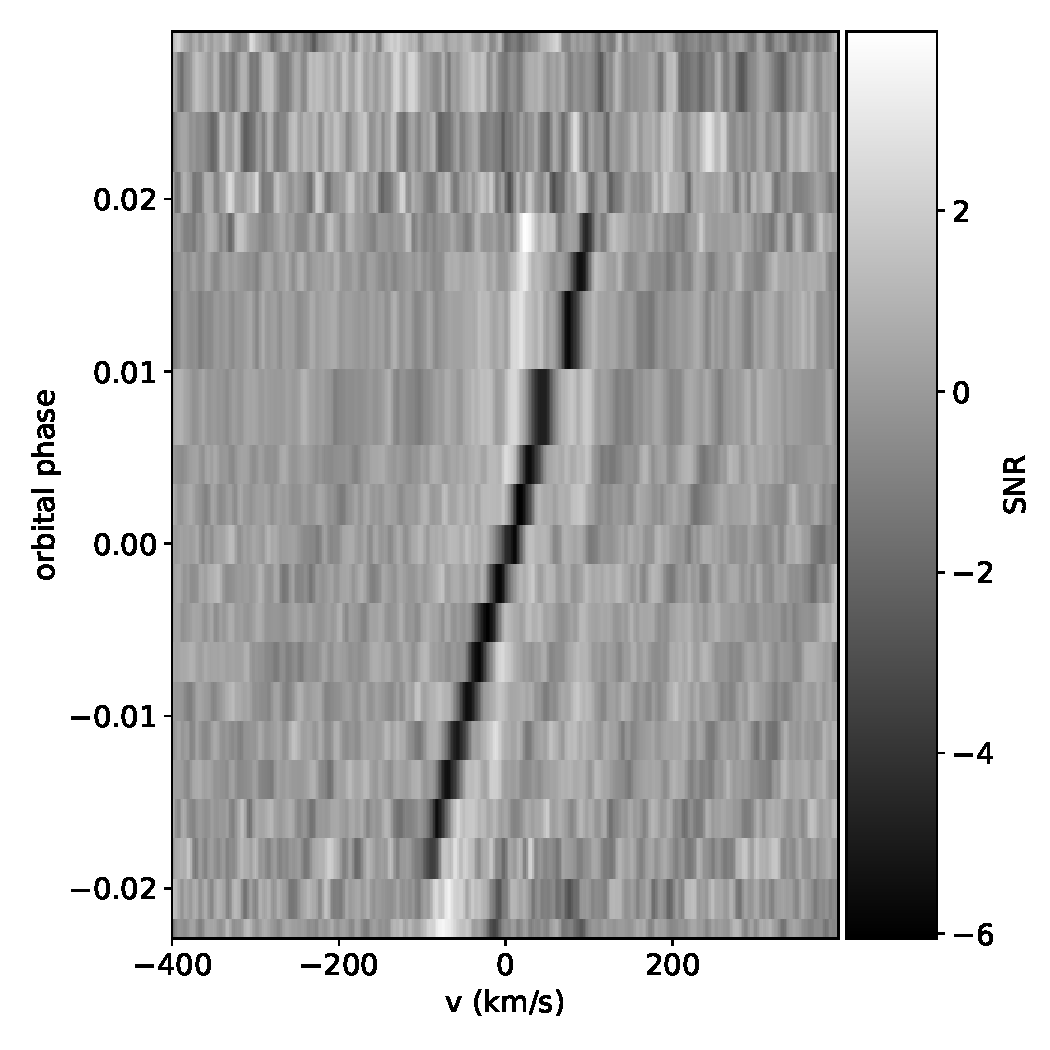
\includegraphics[width=0.45\textwidth]{plots/raw-ccf-before/KELT-20b.20190504.Fe.blue.CCFs-raw.pdf}
                    \hspace{0.05\textwidth}
                    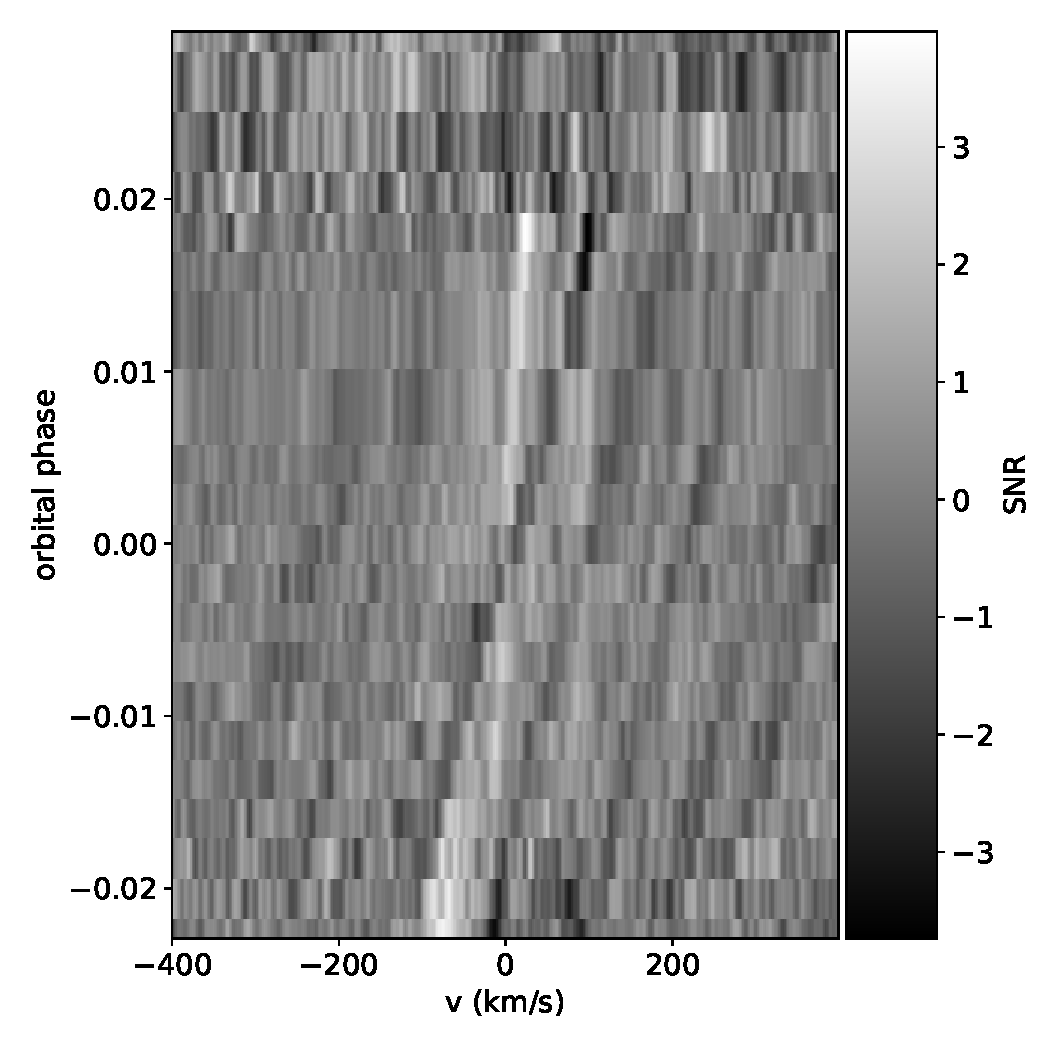
\includegraphics[width=0.45\textwidth]{plots/raw-ccf-after/KELT-20b.20190504.Fe.blue.CCFs-raw.pdf}
                    \caption{Removal of the Doppler shadow in the blue arm CCF of Fe I. \textit{Left panel}: CCF of in-transit exposures showing Doppler Shadow (dark streak) intersecting with the radial velocity signal (bright streak). \textit{Right panel}: Residual CCF after subtracting off the Doppler shadow.}
                    \label{fig:doppler-shadow-removal}
                \end{figure}
            
        \subsection{Line Velocities}\label{subsec:Line Velocities}
            The fitting procedure is as follows: Working in the ${K_p-\Delta\!V}$ space of a single time-series CCF, we loop over a range of possible $K_p$ values: $50$-$350$. For each $K_p$ slice, we search through the peaks along the one-dimensional $RV$ array in descending order, selecting the greatest peak with an $|RV| \leq 15$ kms$^{-1}$. We then fit the Gaussian curve, our initial guess for its center $\mu = RV$. This procedure automatically filters out peaks at nonphysical velocities that may arise due to aliasing.
            
            We select the fit parameters corresponding to the $K_p$ slice hosting the peak CCF amplitude across the entire $K_p-\Delta V$ map, reporting the species velocity $v_{sys} = \mu$ and its detection significance $SNR$ equal to the amplitude of the Gaussian in Table~\ref{tab:results-summary}.
            
            We repeat this fitting procedure for each in-transit time-series CCF, but instead selecting the fit parameters that correspond to the $K_p$ slice equal to the expected $K_p$ of KELT-20b per the ephemeris in Table~\ref{tab:parameters_summary}. We then plot the species' $\Delta V$ as a function of orbital phase, effectively observing its line velocity change over the course of each in-transit exposure. The described plots for each species are in Figure~\ref{fig:Detections}. 

        \subsection{Assessing Detection Validity}\label{subsec:Assessing Detection Results}
            With a ${K_p-\Delta V}$ map 2D CCF, 1D CCF with Gaussian fit at peak SNR $K_p$ slice, and a phase-resolved line profile center during transit, we have a comprehensive profile of each atomic species detected in KELT-20b's atmosphere. We heuristically assess the detection validity by noting the location and magnitude of the peak signal on the ${K_p-\Delta V}$ map, and checking three criteria in order: A $>{3\sigma}$ SNR peak, a standard shape within ${K_p-\Delta V}$ space, and a $\Delta V$ within a physical range of line velocities. Aside from this procedure, we must also consider aliasing between the search species and strong lines corresponding to other species in the spectrum, as described in~\citet{Borsato2023}. In the 1D CCFs, these artifacts manifest as peaks at both visually detectable nonphysical $v_{sys}$ values, and peaks that overlap with the true absorption signal.
            % plot of example telluric corrections by molecfit
            
            % plots showing petitRADTRANS-generated model spectra for each species meeting tentative detection threshold
            
    \section{Results}\label{sec:Results}

        \begin{deluxetable*}{lcccccccc}\label{tab:detection-summary}
            \tablecaption{}
            \tablehead{
                \colhead{} & 
                \colhead{Spectrograph} & 
                \colhead{Arm} &
                \colhead{$N_{\text{obs}}$} &
                \colhead{Species} & 
                \colhead{SNR ($\sigma$)} & 
                \colhead{$\Delta V$ (kms$^{-1}$)}& 
                \colhead{FWHM (kms$^{-1}$)} &
                \colhead{$K_p$ (kms$^{-1}$)}
            }
            \startdata
                \textbf{This Work} & PEPSI & Blue & 1 & Mg I & $5.41 \pm 0.36$ & $3.11 \pm 0.69$ & $21.35 \pm 1.62$ & $177$ \\
                & & Combined & & Fe I & $7.09 \pm 0.56$ & $1.88 \pm 0.44$ & $11.37 \pm 1.05$ & $188$ \\
                & & Combined & & Fe II & $12.48 \pm 0.73$ & $2.83 \pm 0.24$ & $8.56 \pm 0.57$ & $163$ \\
                & & Combined & & Na I & $4.43 \pm 0.60$ & $6.59 \pm 0.53$ & $8.01 \pm 1.24$ & $249$ \\
                & & Combined & & Cr I & $3.47 \pm 0.48$ & $-1.08 \pm 0.75$ & $11.07 \pm 1.77$ & $249$ \\
                & & Blue & & Cr II & $4.15 \pm 0.49$ & $2.00 \pm 0.74$ & $12.77 \pm 1.74$ & $221$ \\
                & & Blue & & Co I & $3.70 \pm 0.52$ & $0.93 \pm 0.49$ & $7.05 \pm 1.15$ & $123$ \\
                & & Blue & & Zn I & $3.19 \pm 0.56$ & $6.48 \pm 0.62$ & $7.18 \pm 1.44$ & $187$ \\
                & & Blue & & Ca I & $3.41 \pm 0.48$ & $6.29 \pm 0.57$ & $10.34 \pm 1.34$ & $211$ \\
                & & Blue & & Cu I & $4.00 \pm 0.50$ & $8.19 \pm 0.59$ & $9.69 \pm 1.39$ & $189$ \\
                & & Blue & & Ti II & $3.04 \pm 0.63$ & $5.94 \pm 0.69$ & $6.77 \pm 1.63$ & $239$ \\
                \citet{CasasayasBarris2019} & HARPS-N & --- & 3 & Fe II & --- & $-2.8 \pm 0.8$ & $7.2 \pm 1.2$ & $174.4 \pm 14.0$ \\
                & & --- & & Na I & --- & $-3.1 \pm 0.9$ & $9.2 \pm 2.0$ & $176.6 \pm 11.7$ \\
                & & --- & & $H_{\alpha}$ & --- & $-3.0 \pm 1.2$ & $19.0 \pm 1.6$ & $165.6 \pm 16.7$ \\
                & & --- & & $H_{\beta}$ & --- & $-1.2 \pm 1.4$ & $19.4 \pm 2.5$ & $136.2 \pm 18.6$ \\
                & & --- & & $H_{\gamma}$ & --- & $-2.3 \pm 2.7$  & $16.6 \pm 4.2$ & $135.0 \pm 34.8$ \\
                & CARMENES & --- & 1 & Na I & --- & $-3.2 \pm 1.7$ & $8.0 \pm 1.2$ & $182.5 \pm 14.3$ \\
                & & --- & & Ca II & --- & $-1.9 \pm 0.6$ & $9.2 \pm 1.0$ & $157.7 \pm 8.2$ \\
                & & --- & & $H_{\alpha}$ & --- & $-4.5 \pm 0.5 $ & $22.6 \pm 0.9 $ & $166.2 \pm 7.4$ \\
                \citet{Hoeijmakers2020} & EXPRES & --- & 1 & Fe I & $3.45$ & $-4.81 \pm 0.72$ & $12.39 \pm 1.69$ & 175 \\
                & & --- & & Fe II & $4.60$ & $-0.75 \pm 0.37$ & $8.54 \pm 0.87$ & 175 \\
                & & --- & & Cr II & $3.69$ & $-3.40 \pm 0.42$ & $5.31 \pm 0.99$ & 175 \\
                & & --- & & Na I & $3.40$ & $-4.38 \pm 0.54$ & $10.07 \pm 1.26$ & 175 \\
                & & --- & & Mg I & $3.33$ & $-8.40 \pm 1.40$ & $33.45 \pm 3.30$ & 175 \\
                \citet{Nugroho2020} & HARPS-N & --- & 3 & Fe I & $14.30$ & $-3.6 \pm 0.3$ & & $200.1 \pm 5.2$ \\
                & & --- & & Fe II & $14.61$ & $-1.4 \pm 0.2$ & & $165.0 \pm 3.5$ \\
                & & --- & & Na I & $7.72$ & $-1.4 \pm 0.7$ & & $180.0 \pm 11.8$ \\
                & & --- & & Ca II & $7.53$ & $2.2 \pm 1.2$ &  & $138.5 \pm 15.3$\\
                & CARMENES & --- & 1 & Fe I & $6.44$ & $-6.5 \pm 0.6$ &  & $263.1 \pm 8.8$\\
                &          & --- &   & Fe II &$3.60$ & $-0.4 \pm 0.6$ &  & $139.2 \pm 2.5$\\
                &          & --- &   & Na I  &$6.83$ & $-0.6 \pm 0.7$ &  & $167.3 \pm 12.1$\\
                &          & --- &   & Ca II &$8.60$ & $0.1 \pm 0.6$ &   & $174.8 \pm 8.2$ \\
                \citet{Rainer2021} & HARPS-N & --- & 5 & Fe I & --- & $-4.7^{+0.3}_{-0.7}$ &  & $147^{+7}_{-6}$\\
                \citet{Langeveld2022} & HARPS-N & --- & 3 & Na I & --- & $-3.1 \pm 1.9$ & --- & \\
                \citet{Sicilia2022} & HARPS-N & --- & 3 & $H_{\alpha}$ & --- & $-5.2^{+1.8}_{-1.7}$ & $27.9^{+3.7}_{-3.3}$ &$156.3^{+28.5}_{-27.0}$ \\
                & & --- & & Na I D$_1$ & --- & $-3.8^{+0.7}_{-0.7}$ & $12.5^{+2.9}_{-2.3}$ & $192.5^{+12.4}_{-13.5}$\\
                & & --- & & Na I D$_2$ & --- & $-3.7^{+0.9}_{-0.9}$ & $14.8^{+2.8}_{-2.4}$ & $170.0^{+14.9}_{-13.5}$\\
            \enddata
        \end{deluxetable*}
        
        \subsection{Detections and Nondetections}\label{subsec:Detections}

        To date, high-resolution cross-correlation transmission spectroscopy (HRCCTS) of KELT-20b has yielded detections of Mg I, Fe I, Fe II, Na I, Cr II, and Ca II \citep{CasasayasBarris2019, Hoeijmakers2020, Nugroho2020, Rainer2021, Langeveld2022, Sicilia2022}, all of which we confirm. Additionally, we present a novel detection of Cu I and tentative detections of Cr I, Co I, Zn I, Ca I, and Ti II. 

        The first step in our detection methodology is to determine which arm(s) of the spectrograph and subsequent cross-correlations to analyze. First, we examine generated transmission spectra

        \begin{figure}
            \centering
            \gridline{
                        \fig{plots-updated/spectra/spectrum.KELT-20b.Fe+.5.395650007488179e-05.inverted-transmission-better.pdf}{0.25\textwidth}{}
                        \fig{plots-updated/line-profile-overlaidarms/KELT-20b.20190504.combined.Fe II.line-profiles-overlaidarms.pdf}{0.25\textwidth}{}
            }
            \gridline{
                        \fig{plots-updated/spectra/spectrum.KELT-20b.Mg.6.08e-05.inverted-transmission-better.pdf}{0.25\textwidth}{}
                        \fig{plots-updated/line-profile-overlaidarms/KELT-20b.20190504.combined.Mg I.line-profiles-overlaidarms.pdf}{0.25\textwidth}{}
            }
            \label{fig:enter-label}
        \end{figure}



        
        
        
        The cross-correlation map of each species, with the dark streak being the atmospheric signal, can be found in the first column of Figure \ref{fig:Detections} for each species. The $K_p - \delta V$ map of each is in the second column, and the 1D CCF of each is in the third column. We 
        
        
        (see Table \ref{tab:detection-summary} and Figure \ref{fig:Detections}).
        \subsection{Atmospheric Dynamics}\label{subsec:Atmospheric Dynamics}

        We seek to disentangle the various atmospheric dynamical mechanisms of KELT-20b by analyzing the phase-resolved line profiles of each species. We compare the offset of the center of the Gaussian fit to the line velocity from zero velocity in the planetary rest frame ($K_p -RV$ or $\Delta V$) between ingress and egress ($phi < 0$ and $phi > 0$) and the phase-binned $\Delta V$) over the course of transit. For species exceeding the detection threshold ($4 \sigma$) in each exposure, we offer a comprehensive view of the planet's dynamics during this observation. By comparing our results to previous works \citep{}, we also provide evidence for dynamical evolution.

        With the line behavior analyzed over the course of transit, we are left to attribute the observed asymmetries to several atmospheric equilibrium mechanisms. These include, but are not limited to, atmospheric escape, scale height differences, condensation, eccentricity, clouds, spatially varying winds, tidal deformation, and temperature-dependent opacity~\citep{Savel2023}. 

        When comparing our HRCCTS observations to models, our conclusions' validity are dependent on the accuracy of the atmospheric model. Given the impact that three-dimensional equilibrium processes, such as those mentioned above, have on $K_p-v_{sys}$ maps~\citep{Wardenier2021}, we wish to provide evidence for one or more of these proposed equilibrium mechanisms and constrain the three-dimensional behavior in the atmosphere for further study. We investigate the phase-dependent dynamics of our detected species in three ways: (1) phase-binning three adjacent in-transit CCFs, ultimately offering seven binned CCFs showing the evolution of the line center, or $\Delta V$ over the course of transit; (2) combining the CCFs into two phase bins -- first contact to second contact and third contact to fourth contact (ingress and egress) -- then plotting each line profile; (3) combining the CCFs into two bins -- first contact to mid-transit and mid-transit to fourth contact -- then plotting each line profile. If present, we can diagnose the drivers of limb asymmetries for each species with two levels of granularity. We limit method (1) to the species exceeding the detection threshold, Mg I, Fe I, Fe II, Na I, Cr II, and Cu I, as the remaining species do not maintain a meaningful signal in the smaller phase bins over the course of transit (see Figure \ref{fig:line-profile-asymmetries} for small bin phase-resolved line profiles of species not shown in this section). We employ methods (2) and (3) for all species, though only some reach the tentative detection threshold in both ingress and egress (see Figure \ref{fig:phase-binned+RVs-results}).

        
                

                    
        \subsection{Nondetections}\label{subsec:Nondetections}

    \section{Conclusions}\label{sec:Conclusions}


    \vspace{5mm}
    \facilities{LBT}

    \software{astropy \citep{astropy}, 
            Jupyter \citep{jupyter},
            matplotlib \citep{Matplotlib},
            molecfit \citep{Kausch2015, Smette2015},
            numpy \citep{NumPy},
            petitRADTRANS \citep{petitRADTRANS},
            PyFastChem \citep{PyFastChem},
            uncertainties~\citet{uncertainties}
            }

    %% Appendix material should be preceded with a single \appendix command.
    %% There should be a \section command for each appendix. Mark appendix
    %% subsections with the same markup you use in the main body of the paper.

    %% Each Appendix (indicated with \section) will be lettered A, B, C, etc.
    %% The equation counter will reset when it encounters the \appendix
    %% command and will number appendix equations (A1), (A2), etc. The
    %% Figure and Table counter will not reset.

\appendix  

    \section{Model transmission spectra}
    \begin{figure}
        \label{fig:model-spectra-appendix}
        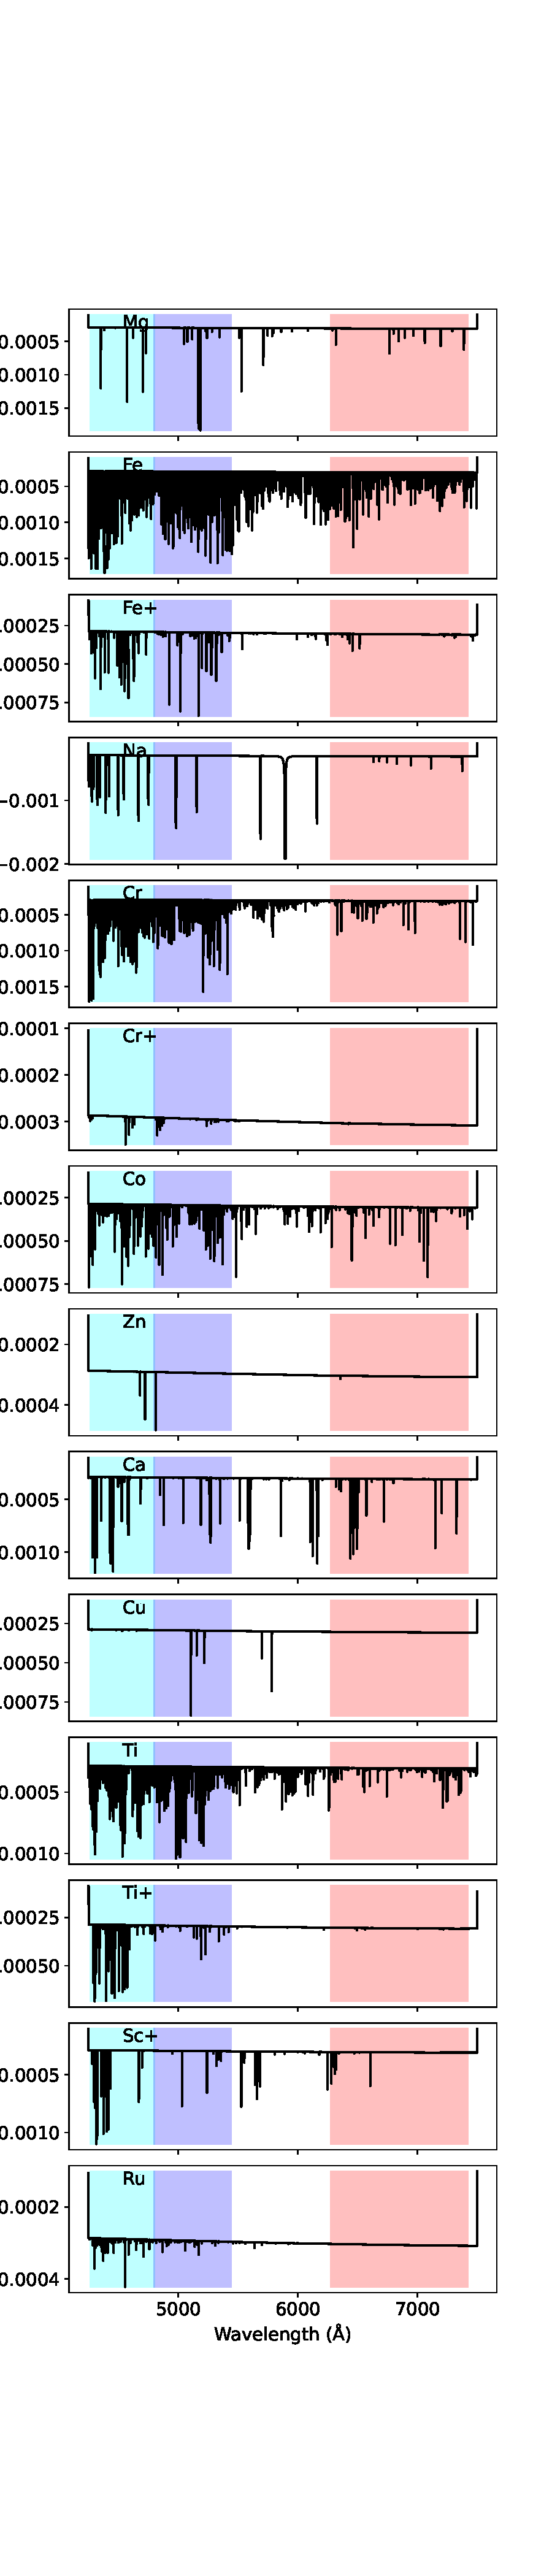
\includegraphics[width=0.4\textwidth]{plots-updated/spectra/spectra.KELT-20b.inverted-transmission-better.pdf}
        % Add additional subfigures as needed
    \caption{Model transmission spectra generated by \code{petitRADTRANS}, with the wavelengths covered by PEPSI's arms shown in blue and red, respectively.}
            
        \end{figure}    


   \section{Detections}

        \begin{figure}
            \label{fig:raw-ccfs-appendix}
            \centering
            \gridline{
                \fig{plots-updated/line-profile-overlaidarms/KELT-20b.20190504.combined.Mg I.line-profiles-overlaidarms.pdf}{0.25\textwidth}{}
                \fig{plots-updated/raw-ccfs/blue/KELT-20b.20190504.Mg.blue.CCFs-raw.pdf}{0.25\textwidth}{\label{fig:raw-ccf-Mg-blue}}
                \fig{plots-updated/kp-vsys-map/blue/KELT-20b.20190504.blue.Mg.CCFs-shifted.pdf}{0.25\textwidth}{\label{fig:2d-ccf-Mg-blue}}
                \fig{plots-updated/line-profile/blue/KELT-20b.20190504.blue.Mg.SNR-Gaussian.pdf}{0.25\textwidth}{\label{fig:1d-ccf-Mg-blue}}
            }
            \gridline{
                \fig{plots-updated/line-profile-overlaidarms/KELT-20b.20190504.combined.Fe I.line-profiles-overlaidarms.pdf}{0.25\textwidth}{}
                \fig{plots-updated/raw-ccfs/combined/KELT-20b.combined.Fe..CCFs-raw.pdf}{0.25\textwidth}{\label{fig:raw-ccf-Fe-blue}}
                \fig{plots-updated/kp-vsys-map/combined/KELT-20b.20190504.combined.Fe.CCFs-shifted.pdf}{0.25\textwidth}{\label{fig:2d-ccf-Fe-combined}}
                \fig{plots-updated/line-profile/combined/KELT-20b.20190504.combined.Fe.SNR-Gaussian.pdf}{0.25\textwidth}{\label{fig:1d-ccf-Fe-combined}}
            }
            \gridline{
                \fig{plots-updated/line-profile-overlaidarms/KELT-20b.20190504.combined.Fe II.line-profiles-overlaidarms.pdf}{0.25\textwidth}{}
                \fig{plots-updated/raw-ccfs/combined/KELT-20b.combined.Fe+..CCFs-raw.pdf}{0.25\textwidth}{\label{fig:raw-ccf-FeII-combined}}
                \fig{plots-updated/kp-vsys-map/combined/KELT-20b.20190504.combined.Fe+.CCFs-shifted.pdf}{0.25\textwidth}{\label{fig:2d-ccf-FeII-combined}}
                \fig{plots-updated/line-profile/combined/KELT-20b.20190504.combined.Fe+.SNR-Gaussian.pdf}{0.25\textwidth}{\label{fig:1d-ccf-FeII-combined}}
            }
            \gridline{
                \fig{plots-updated/line-profile-overlaidarms/KELT-20b.20190504.combined.Na I.line-profiles-overlaidarms.pdf}{0.25\textwidth}{}
                \fig{plots-updated/raw-ccfs/combined/KELT-20b.combined.Na..CCFs-raw.pdf}{0.25\textwidth}{\label{fig:raw-ccf-Na-combined}}
                \fig{plots-updated/kp-vsys-map/combined/KELT-20b.20190504.combined.Na.CCFs-shifted.pdf}{0.25\textwidth}{\label{fig:2d-ccf-Na-combined}}
                \fig{plots-updated/line-profile/combined/KELT-20b.20190504.combined.Na.SNR-Gaussian.pdf}{0.25\textwidth}{\label{fig:1d-ccf-Na-combined}}
            }
        \end{figure}
        
        \begin{figure}
            \gridline{
                \fig{plots-updated/line-profile-overlaidarms/KELT-20b.20190504.combined.Co I.line-profiles-overlaidarms.pdf}{0.25\textwidth}{}
                \fig{plots-updated/raw-ccfs/combined/KELT-20b.combined.Co..CCFs-raw.pdf}{0.25\textwidth}{\label{fig:raw-ccf-Co-combined}}
                \fig{plots-updated/kp-vsys-map/blue/KELT-20b.20190504.blue.Co.CCFs-shifted.pdf}{0.25\textwidth}{\label{fig:2d-ccf-Co-blue}}
                \fig{plots-updated/line-profile/blue/KELT-20b.20190504.blue.Co.SNR-Gaussian.pdf}{0.25\textwidth}{\label{fig:1d-ccf-Co-blue}}
            }
            \gridline{
                \fig{plots-updated/line-profile-overlaidarms/KELT-20b.20190504.combined.Cr I.line-profiles-overlaidarms.pdf}{0.25\textwidth}{}
                \fig{plots-updated/raw-ccfs/combined/KELT-20b.combined.Cr..CCFs-raw.pdf}{0.25\textwidth}{\label{fig:raw-ccf-Cr-combined}}
                \fig{plots-updated/kp-vsys-map/combined/KELT-20b.20190504.combined.Cr.CCFs-shifted.pdf}{0.25\textwidth}{\label{fig:2d-ccf-Cr-combined}}
                \fig{plots-updated/line-profile/combined/KELT-20b.20190504.combined.Cr.SNR-Gaussian.pdf}{0.25\textwidth}{\label{fig:1d-ccf-Cr-combined}}
            }
            \gridline{
                \fig{plots-updated/line-profile-overlaidarms/KELT-20b.20190504.combined.Cr II.line-profiles-overlaidarms.pdf}{0.25\textwidth}{}
                \fig{plots-updated/raw-ccfs/blue/KELT-20b.20190504.Cr+.blue.CCFs-raw.pdf}{0.25\textwidth}{\label{fig:raw-ccf-CrII-blue}}
                \fig{plots-updated/kp-vsys-map/blue/KELT-20b.20190504.blue.Cr+.CCFs-shifted.pdf}{0.25\textwidth}{\label{fig:2d-ccf-CrII-blue}}
                \fig{plots-updated/line-profile/blue/KELT-20b.20190504.blue.Cr+.SNR-Gaussian.pdf}{0.25\textwidth}{\label{fig:1d-ccf-CrII-blue}}
            }
            \gridline{
                \fig{plots-updated/line-profile-overlaidarms/KELT-20b.20190504.combined.Zn I.line-profiles-overlaidarms.pdf}{0.25\textwidth}{}
                \fig{plots-updated/raw-ccfs/blue/KELT-20b.20190504.Zn.blue.CCFs-raw.pdf}{0.25\textwidth}{\label{fig:raw-ccf-Zn-blue}}
                \fig{plots-updated/kp-vsys-map/blue/KELT-20b.20190504.blue.Zn.CCFs-shifted.pdf}{0.25\textwidth}{\label{fig:2d-ccf-Zn-blue}}
                \fig{plots-updated/line-profile/blue/KELT-20b.20190504.blue.Zn.SNR-Gaussian.pdf}{0.25\textwidth}{\label{fig:1d-ccf-Zn-blue}}
            }
        \end{figure}
        
        \begin{figure}
            \gridline{
                \fig{plots-updated/line-profile-overlaidarms/KELT-20b.20190504.combined.Cu I.line-profiles-overlaidarms.pdf}{0.25\textwidth}{}
                \fig{plots-updated/raw-ccfs/blue/KELT-20b.20190504.Cu.blue.CCFs-raw.pdf}{0.25\textwidth}{\label{fig:raw-ccf-Cu-blue}}
                \fig{plots-updated/kp-vsys-map/blue/KELT-20b.20190504.blue.Cu.CCFs-shifted.pdf}{0.25\textwidth}{\label{fig:2d-ccf-Cu-blue}}
                \fig{plots-updated/line-profile/blue/KELT-20b.20190504.blue.Cu.SNR-Gaussian.pdf}{0.25\textwidth}{\label{fig:1d-ccf-Cu-blue}}
            }
            \gridline{
                \fig{plots-updated/line-profile-overlaidarms/KELT-20b.20190504.combined.Ca I.line-profiles-overlaidarms.pdf}{0.25\textwidth}{}
                \fig{plots-updated/raw-ccfs/blue/KELT-20b.20190504.Ca.blue.CCFs-raw.pdf}{0.25\textwidth}{\label{fig:raw-ccf-Ca-blue}}
                \fig{plots-updated/kp-vsys-map/blue/KELT-20b.20190504.blue.Ca.CCFs-shifted.pdf}{0.25\textwidth}{\label{fig:2d-ccf-Ca-blue}}
                \fig{plots-updated/line-profile/blue/KELT-20b.20190504.blue.Ca.SNR-Gaussian.pdf}{0.25\textwidth}{\label{fig:1d-ccf-Ca-blue}}
            }
            \gridline{
                \fig{plots-updated/line-profile-overlaidarms/KELT-20b.20190504.combined.Ti II.line-profiles-overlaidarms.pdf}{0.25\textwidth}{}
                \fig{plots-updated/raw-ccfs/blue/KELT-20b.20190504.Ti+.blue.CCFs-raw.pdf}{0.25\textwidth}{\label{fig:raw-ccf-TiII-blue}}
                \fig{plots-updated/kp-vsys-map/blue/KELT-20b.20190504.blue.Ti+.CCFs-shifted.pdf}{0.25\textwidth}{\label{fig:2d-ccf-TiII-blue}}
                \fig{plots-updated/line-profile/blue/KELT-20b.20190504.blue.Ti+.SNR-Gaussian.pdf}{0.25\textwidth}{\label{fig:1d-ccf-TiII-blue}}
            }
            \caption{Cross-correlation results for each detected and tentatively detected atomic species in our analysis. \textit{Left panel}: $K_p-RV$ maps in the stellar rest frame. \textit{Middle panel}: $K_p-\Delta V$ maps, shifted into the planetary rest frame. \textit{Right panel}: $SNR-\Delta V$ map at the $K_p$ corresponding to peak signal. This figure shows the maps, 1D CCFs, and line profiles for each species exceeding the ${3\sigma}$ tentative detection threshold. The offset of the center of the 1D CCF Gaussian from the planetary rest frame, ${v_{sys}}=0$, denotes the line velocity.}
        \end{figure}
        
    \section{Dynamics}
    
        \begin{figure}
            \centering
            \gridline{
                \fig{plots-updated/line-profile-asymmetries/ingress-egress/blue/KELT-20b.20190504.blue.Mg.SNR-Gaussian-Asymmetry.pdf}{0.33\textwidth}{}
                \fig{plots-updated/line-profile-asymmetries/halves/blue/KELT-20b.20190504.blue.Mg.SNR-Gaussian-Asymmetry.pdf}{0.33\textwidth}{}
                \fig{plots-updated/line-velocity/blue/KELT-20b.Mg.blue.phase-binned+RVs.pdf}{0.33\textwidth}{}
            }
            \gridline{
                \fig{plots-updated/line-profile-asymmetries/ingress-egress/blue/KELT-20b.20190504.blue.Fe.SNR-Gaussian-Asymmetry.pdf}{0.33\textwidth}{}
                \fig{plots-updated/line-profile-asymmetries/halves/blue/KELT-20b.20190504.blue.Fe.SNR-Gaussian-Asymmetry.pdf}{0.33\textwidth}{}
                \fig{plots-updated/line-velocity/blue/KELT-20b.Fe.blue.phase-binned+RVs.pdf}{0.33\textwidth}{}
            }
            \gridline{
                \fig{plots-updated/line-profile-asymmetries/ingress-egress/blue/KELT-20b.20190504.blue.Fe+.SNR-Gaussian-Asymmetry.pdf}{0.33\textwidth}{}
                \fig{plots-updated/line-profile-asymmetries/halves/blue/KELT-20b.20190504.blue.Fe+.SNR-Gaussian-Asymmetry.pdf}{0.33\textwidth}{}
                \fig{plots-updated/line-velocity/blue/KELT-20b.Fe+.blue.phase-binned+RVs.pdf}{0.33\textwidth}{}
            }
            \gridline{
                \fig{plots-updated/line-profile-asymmetries/ingress-egress/blue/KELT-20b.20190504.blue.Na.SNR-Gaussian-Asymmetry.pdf}{0.33\textwidth}{}
                \fig{plots-updated/line-profile-asymmetries/halves/blue/KELT-20b.20190504.blue.Na.SNR-Gaussian-Asymmetry.pdf}{0.33\textwidth}{}
                \fig{plots-updated/line-velocity/blue/KELT-20b.Na.blue.phase-binned+RVs.pdf}{0.33\textwidth}{}
            }

        \end{figure}
        \begin{figure}
            \gridline{
                \fig{plots-updated/line-profile-asymmetries/ingress-egress/blue/KELT-20b.20190504.blue.Cr.SNR-Gaussian-Asymmetry.pdf}{0.33\textwidth}{}
                \fig{plots-updated/line-profile-asymmetries/halves/blue/KELT-20b.20190504.blue.Cr.SNR-Gaussian-Asymmetry.pdf}{0.33\textwidth}{}
                \fig{plots-updated/line-velocity/blue/KELT-20b.Cr.blue.phase-binned+RVs.pdf}{0.33\textwidth}{}
            }
            \gridline{
                \fig{plots-updated/line-profile-asymmetries/ingress-egress/blue/KELT-20b.20190504.blue.Cr+.SNR-Gaussian-Asymmetry.pdf}{0.33\textwidth}{}
                \fig{plots-updated/line-profile-asymmetries/halves/blue/KELT-20b.20190504.blue.Cr+.SNR-Gaussian-Asymmetry.pdf}{0.33\textwidth}{}
                \fig{plots-updated/line-velocity/blue/KELT-20b.Cr+.blue.phase-binned+RVs.pdf}{0.33\textwidth}{}
            }
            \gridline{
                \fig{plots-updated/line-profile-asymmetries/ingress-egress/blue/KELT-20b.20190504.blue.Co.SNR-Gaussian-Asymmetry.pdf}{0.33\textwidth}{}
                \fig{plots-updated/line-profile-asymmetries/halves/blue/KELT-20b.20190504.blue.Co.SNR-Gaussian-Asymmetry.pdf}{0.33\textwidth}{}
                \fig{plots-updated/line-velocity/blue/KELT-20b.Co.blue.phase-binned+RVs.pdf}{0.33\textwidth}{}
            }
            \gridline{
                \fig{plots-updated/line-profile-asymmetries/ingress-egress/blue/KELT-20b.20190504.blue.Zn.SNR-Gaussian-Asymmetry.pdf}{0.33\textwidth}{}
                \fig{plots-updated/line-profile-asymmetries/halves/blue/KELT-20b.20190504.blue.Zn.SNR-Gaussian-Asymmetry.pdf}{0.33\textwidth}{}
                \fig{plots-updated/line-velocity/blue/KELT-20b.Zn.blue.phase-binned+RVs.pdf}{0.33\textwidth}{}
            }

        \end{figure}
        \begin{figure}
            \gridline{
                \fig{plots-updated/line-profile-asymmetries/ingress-egress/blue/KELT-20b.20190504.blue.Ca.SNR-Gaussian-Asymmetry.pdf}{0.33\textwidth}{}
                \fig{plots-updated/line-profile-asymmetries/halves/blue/KELT-20b.20190504.blue.Ca.SNR-Gaussian-Asymmetry.pdf}{0.33\textwidth}{}
                \fig{plots-updated/line-velocity/blue/KELT-20b.Ca.blue.phase-binned+RVs.pdf}{0.33\textwidth}{}
            }
            \gridline{
                \fig{plots-updated/line-profile-asymmetries/ingress-egress/blue/KELT-20b.20190504.blue.Cu.SNR-Gaussian-Asymmetry.pdf}{0.33\textwidth}{}
                \fig{plots-updated/line-profile-asymmetries/halves/blue/KELT-20b.20190504.blue.Cu.SNR-Gaussian-Asymmetry.pdf}{0.33\textwidth}{}
                \fig{plots-updated/line-velocity/blue/KELT-20b.Cu.blue.phase-binned+RVs.pdf}{0.33\textwidth}{}
            }
            \gridline{
                \fig{plots-updated/line-profile-asymmetries/ingress-egress/blue/KELT-20b.20190504.blue.Ti+.SNR-Gaussian-Asymmetry.pdf}{0.33\textwidth}{}
                \fig{plots-updated/line-profile-asymmetries/halves/blue/KELT-20b.20190504.blue.Ti+.SNR-Gaussian-Asymmetry.pdf}{0.33\textwidth}{}
                \fig{plots-updated/line-velocity/blue/KELT-20b.Ti+.blue.phase-binned+RVs.pdf}{0.25\textwidth}{}
            }
            \caption{Phase-binned radial velocity measurements}
            \label{fig:phase-binned+RVs-results}
        \end{figure}
        
        \begin{figure}[]\label{fig:combined-line-profiles-appendix} 
            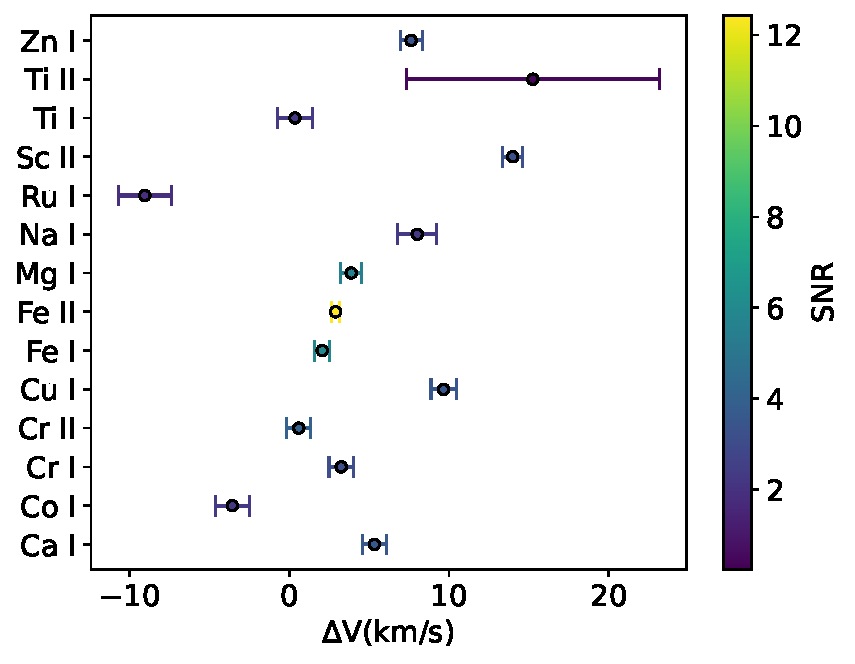
\includegraphics[width=0.45\textwidth]{plots-updated/KELT-20b.inverted-transmission-better.CombinedRVs.pdf}
            \caption{The net Doppler shifts of each detected species, ordered and colored by their peak detection SNR.}
            
        \end{figure}



    \section{Nondetections}
        \begin{figure}
            
            \gridline{
                \fig{plots-updated/raw-ccfs/blue/KELT-20b.20190504.Ru.blue.CCFs-raw.pdf}{0.25\textwidth}{\label{fig:raw-ccf-Mg-blue}}
                \fig{plots-updated/kp-vsys-map/blue/KELT-20b.20190504.blue.Ru.CCFs-shifted.pdf}{0.25\textwidth}{\label{fig:2d-ccf-Fe+-blue}}
                \fig{plots-updated/line-profile/blue/KELT-20b.20190504.blue.Ru.SNR-Gaussian.pdf}{0.25\textwidth}{\label{fig:1d-ccf-Fe+-blue}}
            }
            \gridline{
                \fig{plots-updated/raw-ccfs/blue/KELT-20b.20190504.Ti.blue.CCFs-raw.pdf}{0.25\textwidth}{\label{fig:raw-ccf-Mg-blue}}
                \fig{plots-updated/kp-vsys-map/blue/KELT-20b.20190504.blue.Ti.CCFs-shifted.pdf}{0.25\textwidth}{\label{fig:2d-ccf-Fe+-blue}}
                \fig{plots-updated/line-profile/blue/KELT-20b.20190504.blue.Ti.SNR-Gaussian.pdf}{0.25\textwidth}{\label{fig:1d-ccf-Fe+-blue}}
            }
            \gridline{
                \fig{plots-updated/raw-ccfs/blue/KELT-20b.20190504.Sc+.blue.CCFs-raw.pdf}{0.25\textwidth}{\label{fig:raw-ccf-Mg-blue}}
                \fig{plots-updated/kp-vsys-map/blue/KELT-20b.20190504.blue.Sc+.CCFs-shifted.pdf}{0.25\textwidth}{\label{fig:2d-ccf-Fe+-blue}}
                \fig{plots-updated/line-profile/blue/KELT-20b.20190504.blue.Sc+.SNR-Gaussian.pdf}{0.25\textwidth}{\label{fig:1d-ccf-Fe+-blue}}
            }
            
             \caption{Cross-correlation results for each detected and tentatively detected atomic species in our analysis. \textit{Left panel}: $K_p-RV$ maps in the stellar rest frame. \textit{Middle panel}: $K_p-\Delta V$ maps, shifted into the planetary rest frame.
                            \textit{Left panel}: $SNR-\Delta V$ map at the $K_p$ corresponding to peak signal. This figure shows the  maps, 1D CCFs, and line profiles for each species exceeding the ${3\sigma}$ tentative detection threshold. The offset of the center of the 1D CCF Gaussian from the planetary rest frame, ${v_{sys}}=0$, denotes the line velocity.}
        \end{figure}




\bibliography{bibliography}{}
\bibliographystyle{aasjournal}       
    \clearpage

\end{document}